\documentclass[tikz,border=8pt]{standalone}
% Shared look for every TikZ diagram. Load with \input{../../tools/tikz-style.tex}
\usepackage[T1]{fontenc}
\usepackage{lmodern}
\renewcommand{\sfdefault}{lmr}  % diagrams use the same serif as the text
\usetikzlibrary{arrows.meta, positioning, shapes.geometric, calc, fit, backgrounds}
\definecolor{cblue}{HTML}{4C78A8}
\definecolor{corange}{HTML}{F58518}
\definecolor{cgreen}{HTML}{54A24B}
\definecolor{cred}{HTML}{E45756}
\definecolor{cpurple}{HTML}{B279A2}
\definecolor{cgrey}{HTML}{6B6B6B}
\tikzset{
  every picture/.style={font=\sffamily, line width=1.2pt},
  box/.style={draw=#1, fill=#1!12, rounded corners=4pt, align=center, inner sep=7pt, minimum height=1.1cm},
  box/.default=cgrey,
  arrow/.style={-{Stealth[length=3mm]}, draw=cgrey, line width=1.4pt},
  title/.style={font=\sffamily\bfseries\Large},
  note/.style={font=\sffamily\small, text=cgrey, align=center},
}
\AtBeginDocument{\hyphenpenalty=10000 \exhyphenpenalty=10000}

% A room 7 m x 4 m with a door. The scan says: a flat wall 1 m straight ahead. Every pose 1 m from a straight stretch
% of wall, facing it, fits (blue arrows); near a corner or the door the scan would look different, so those are out.
\begin{document}
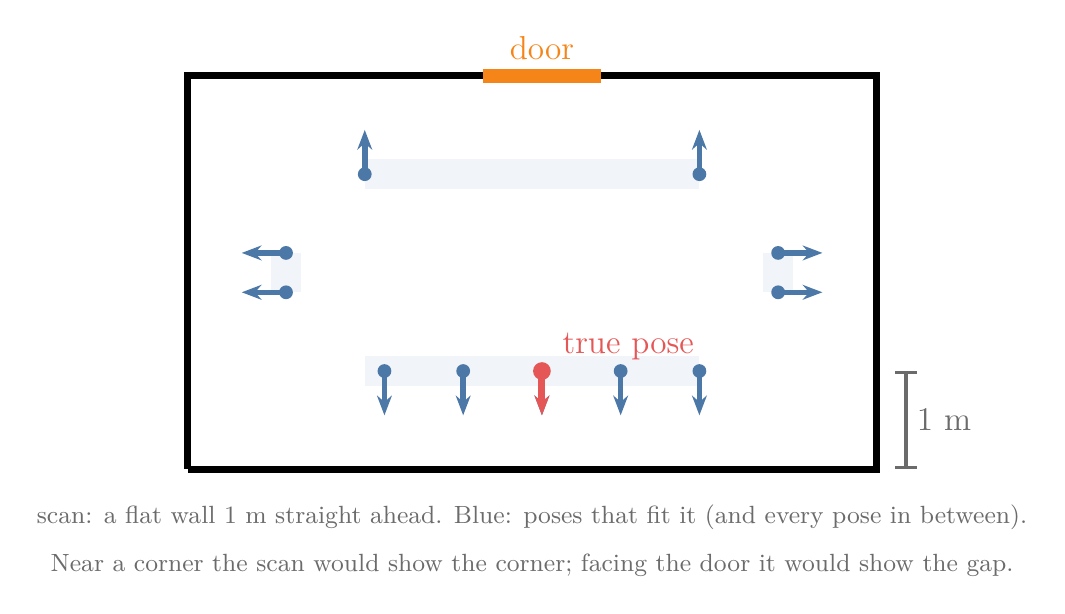
\begin{tikzpicture}[scale=1.25, every node/.append style={font=\large}]
  \fill[cblue!8] (1.8,0.85) rectangle (5.2,1.15);  \fill[cblue!8] (1.8,2.85) rectangle (5.2,3.15);
  \fill[cblue!8] (0.85,1.8) rectangle (1.15,2.2);  \fill[cblue!8] (5.85,1.8) rectangle (6.15,2.2);
  \draw[black, line width=2.5pt] (0,0) -- (7,0) -- (7,4) -- (4.2,4);
  \draw[black, line width=2.5pt] (3.0,4) -- (0,4) -- (0,0);
  \draw[corange, line width=5pt] (3.0,4) -- (4.2,4); \node[corange, above] at (3.6,4.05) {door};
  % candidate poses: 1 m from a wall, facing it
  \foreach \x in {2,2.8,3.6,4.4,5.2} {
    \draw[-{Stealth[length=2.5mm]}, cblue, line width=2pt] (\x,1) -- (\x,0.55); \fill[cblue] (\x,1) circle (0.07);
  }
  \foreach \x in {1.8,5.2} {
    \draw[-{Stealth[length=2.5mm]}, cblue, line width=2pt] (\x,3) -- (\x,3.45); \fill[cblue] (\x,3) circle (0.07);
  }
  \foreach \y in {1.8,2.2} {
    \draw[-{Stealth[length=2.5mm]}, cblue, line width=2pt] (1,\y) -- (0.55,\y); \fill[cblue] (1,\y) circle (0.07);
    \draw[-{Stealth[length=2.5mm]}, cblue, line width=2pt] (6,\y) -- (6.45,\y); \fill[cblue] (6,\y) circle (0.07);
  }
  % true robot
  \draw[-{Stealth[length=2.5mm]}, cred, line width=2.5pt] (3.6,1) -- (3.6,0.55); \fill[cred] (3.6,1) circle (0.09);
  \node[cred, right] at (3.7,1.25) {true pose};
  \draw[cgrey, |-|] (7.3,0) -- (7.3,1) node[midway, right] {1 m};
  \node[note, anchor=north] at (3.5,-0.25) {scan: a flat wall 1 m straight ahead. Blue: poses that fit it (and every pose in between).};
  \node[note, anchor=north] at (3.5,-0.75) {Near a corner the scan would show the corner; facing the door it would show the gap.};
\end{tikzpicture}
\end{document}
